%-------------------------------------------------------------------------
% PACKAGES AND OTHER DOCUMENT CONFIGURATIONS
%-------------------------------------------------------------------------

\documentclass[11pt]{article}
%----------------------------------------------------------------------------------------------
%   PACKAGES AND CONFIGURATIONS 
%----------------------------------------------------------------------------------------------

\usepackage{lastpage}
\usepackage{hyperref}
\usepackage{graphicx}
\usepackage{pgfplots}
\pgfplotsset{compat=1.17}
\usepackage{xcolor}
\usepackage{amsmath}
\usepackage{bussproofs}
\usepackage{amssymb}
\usepackage{amsfonts}
\usepackage{graphicx}
\usepackage{booktabs}
\usepackage{listing}
\usepackage{etoolbox}
\usepackage{latexsym}
\usepackage{listings}
\usepackage[utf8]{inputenc}
\usepackage{caption}
\graphicspath{{./img}}

\DeclareCaptionFont{white}{\color{white}}
\DeclareCaptionFormat{listing}{%
  \parbox{\textwidth}{\colorbox{gray}{\parbox{\textwidth}{#1#2#3}}\vskip-4pt}}
\captionsetup[lstlisting]{format=listing,labelfont=white,textfont=white}
\lstset{frame=lrb,xleftmargin=\fboxsep,xrightmargin=-\fboxsep}

%-----------------------------------------------------------------------------------------------
%   MARGINS
%-----------------------------------------------------------------------------------------------

\usepackage{geometry}
\geometry{
    paper=a4paper,
    top=3cm,
    bottom=3cm,
    left=2.5cm,
    right=2.5cm,
    headheight=14pt,
    footskip=1.4cm,
    headsep=1.2cm,
}

%-----------------------------------------------------------------------------------------------
%   FONT
%-----------------------------------------------------------------------------------------------

\usepackage[utf8]{inputenc}
\usepackage[T1]{fontenc}

\usepackage[sfdefault,light]{roboto}

%-----------------------------------------------------------------------------------------------
%   HEADER AND FOOTER   
%-----------------------------------------------------------------------------------------------

\usepackage{fancyhdr}
\pagestyle{fancy}

\lhead{\small\classHomework\ifdef{\className}{\ (\className):}{}\ \homeworkTitle}
\chead{}
\rhead{\small\ifdef{\authorName}{\authorName}{\ifdef{dueDate}{Due\ \dueDate}{}}}

\lfoot{}
\cfoot{\small Page\ \thepage\ of\ \pageref{LastPage}}
\rfoot{
\includegraphics[scale=0.06]{logo-unige.png}}

\renewcommand\headrulewidth{0.5pt}

%-------------------------------------------------------------------------------------------------
%   TITLE PAGE
%-------------------------------------------------------------------------------------------------

\author{\textbf{\authorName}}
\date{}

\title{
    \thispagestyle{empty}
    \vspace{0.2\textheight}
    \textbf{\classHomework:\ \homeworkTitle}\\[-4pt]
    \ifdef{\classHomework}{{\small Due\ on\ \dueDate}\\}{}
    \ifdef{\className}{{\large \textit{\className}}}{}
    \vspace{0.32\textheight}

    
\includegraphics[scale=0.2]{logo-unige.png}
}
 % Ensure this file contains all necessary package inclusions and settings

%-------------------------------------------------------------------------
% HOMEWORK INFORMATION
%-------------------------------------------------------------------------

\newcommand{\classHomework}{13X007}
\newcommand{\homeworkTitle}{Assignment\ \#5}
\newcommand{\authorName}{CHRISTOFOROU Anthony}
\newcommand{\className}{Parallelism}
\newcommand{\dueDate}{04.12.2023}

%-------------------------------------------------------------------------

\begin{document}
    
    \maketitle
    \thispagestyle{empty}
    \newpage

    \begin{abstract}
        This report delves into the detailed implementation and analysis of the Mandelbrot set generation using OpenMP for parallel computing. We examine the effects of various thread counts and computational regions on performance, providing insights into parallelization strategies and their implications on complex mathematical computations.
    \end{abstract}

    \tableofcontents
    
    \newpage
    
    \section{Introduction}
The Mandelbrot set is a cornerstone in fractal geometry, epitomizing the intricate structures that emerge from simple mathematical rules. Its computation, inherently complex and resource-intensive, presents an ideal case for exploring the capabilities of parallel computing. This report presents a deep dive into the generation of the Mandelbrot set using OpenMP, a widely-used parallel programming framework in C++. We aim to explore how parallel computation can be leveraged to optimize the rendering of this fractal, analyzing the performance across different thread counts and regions of computation.

\section{Methodology}

\subsection{Theory}
The Mandelbrot set is a set of complex numbers defined by a simple iterative formula: For a given complex number \( c \), the sequence \( f_{c}(0) \), \( f_{c}(f_{c}(0)) \), ..., with \( f_{c}(z) = z^2 + c \), remains bounded. The beauty of the Mandelbrot set lies in the complexity and variety of patterns that emerge from this simple definition.
\subsection{Mandelbrot Set Computation}
Our implementation in C++ leverages complex number arithmetic to iterate over points in the complex plane. We evaluate the boundedness of each point under the iterative function, thereby determining its membership in the Mandelbrot set.
\begin{verbatim}
    // Function to check if a point is in the Mandelbrot set
    int isInMandelbrotSet(std::complex<double> c, int maxIterations) {
        std::complex<double> z = 0;
        int n = 0;
        for (n = 0; n < maxIterations; ++n) {
            if (std::abs(z) > 2.0) {
                break;
            }
            z = z * z + c;
        }
        return n;
    }
\end{verbatim}

    This function takes a complex number \texttt{c} and an iteration limit \texttt{maxIterations} as parameters. It initializes a complex number \texttt{z} to zero and iterates \texttt{z} as \texttt{z = z * z + c}. If the magnitude of \texttt{z} exceeds 2, the function terminates, indicating that \texttt{c} does not belong to the Mandelbrot set. The number of iterations before divergence is returned as an indication of how quickly the points diverge.

    \subsection{Parallelization}
Using OpenMP, we distribute this computation across multiple threads. This section will discuss the specific OpenMP directives employed, their configuration, and the rationale behind their use in optimizing the computation process.

\begin{verbatim}
    // Parallel computation of Mandelbrot set
    #pragma omp parallel for private(x, y, c, n)
    for (int i = 0; i < imageHeight; ++i) {
        for (int j = 0; j < imageWidth; ++j) {
            c = std::complex<double>(x_min + j * pixel_size_x,
                                     y_min + i * pixel_size_y);
            n = isInMandelbrotSet(c, maxIterations);
        }
    }
\end{verbatim}
    In this snippet, the \texttt{\#pragma omp parallel for} directive is used to distribute the computation of each pixel in the Mandelbrot set image across multiple threads. Each thread computes a subset of the total pixels, thereby dividing the workload and reducing the overall execution time.

\subsection{Image Rendering}
The computed set is rendered into a BMP image using a custom function, \texttt{write\_to\_bmp}. This function maps the number of iterations required for divergence to a color scale, effectively visualizing the fractal pattern of the Mandelbrot set.

\section{Results}
\subsection{Execution Time vs. Thread Count}
We conducted experiments with varying numbers of threads to analyze the performance of our parallel algorithm. This section provides a detailed examination of the execution times across different thread counts, highlighting the scalability and efficiency of the parallelized implementation.

    \begin{verbatim}
        Execution Time with 1 threads: 0.205807 seconds
        Fractal image saved as BMP.
        Execution Time with 2 threads: 0.101268 seconds
        ...
        Execution Time with 128 threads: 0.0244127 seconds
        Fractal image saved as BMP.
        Execution Time with 256 threads: 0.0308905 seconds
        Fractal image saved as BMP.
    \end{verbatim}

    The execution times show a clear trend: as the thread count increases from 1 to 64, there is a significant reduction in execution time, demonstrating the benefits of parallel computation. However, post 64 threads, there is a slight increase in execution time, indicating a point of diminishing returns.

    % Include the graph for Execution Time vs. Thread Count here
    \begin{center}  
        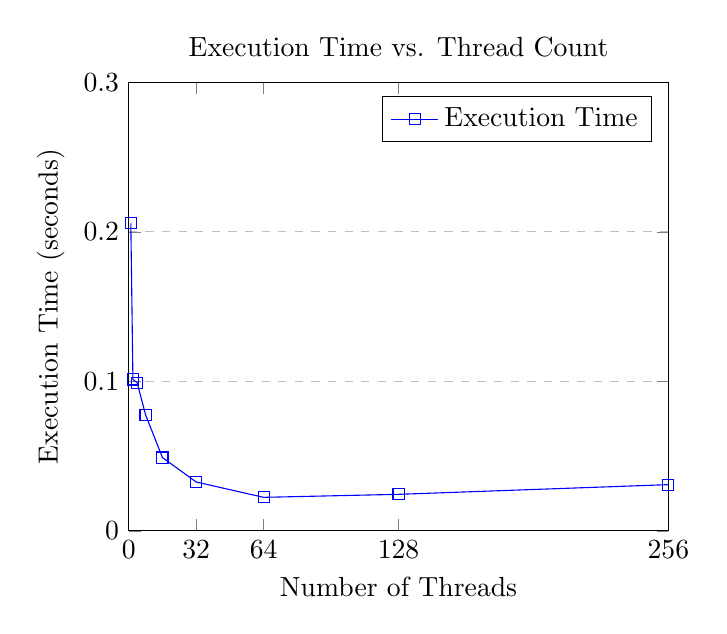
\begin{tikzpicture}
        \begin{axis}[
            title={Execution Time vs. Thread Count},
            xlabel={Number of Threads},
            ylabel={Execution Time (seconds)},
            xmin=0, xmax=256,
            ymin=0, ymax=0.3,
            xtick={0,32,64,128,256},
            ytick={0,0.1,0.2,0.3},
            legend pos=north east,
            ymajorgrids=true,
            grid style=dashed,
        ]
    
        \addplot[
            color=blue,
            mark=square,
            ]
            coordinates {
            (1,0.205807)(2,0.101268)(4,0.0991456)(8,0.0776037)(16,0.0490366)(32,0.0326639)(64,0.022394)(128,0.0244127)(256,0.0308905)
            };
            \legend{Execution Time}
    
        \end{axis}
        \end{tikzpicture}
    \end{center}

\subsection{Visualization}
Here, we present the rendered images of the Mandelbrot set for different iteration counts. The section includes an analysis of the fractal patterns, discussing how they evolve with the increase in iterations and threads.

    % Include the image of the Mandelbrot set here
    \begin{figure}[ht]
        \centering
        
\includegraphics[width=0.2\textwidth]{img/F_0002.png}
        
\includegraphics[width=0.2\textwidth]{img/F_0004.png}
        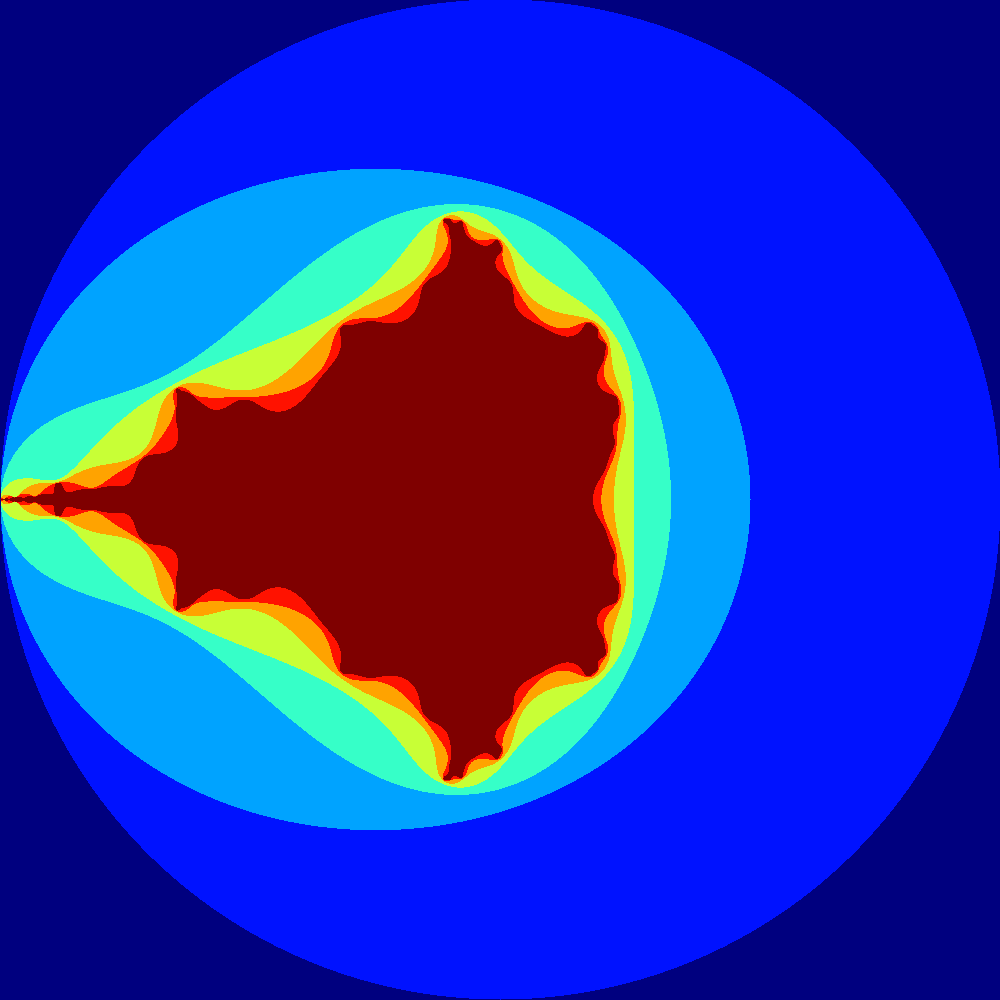
\includegraphics[width=0.2\textwidth]{img/F_0008.png}
        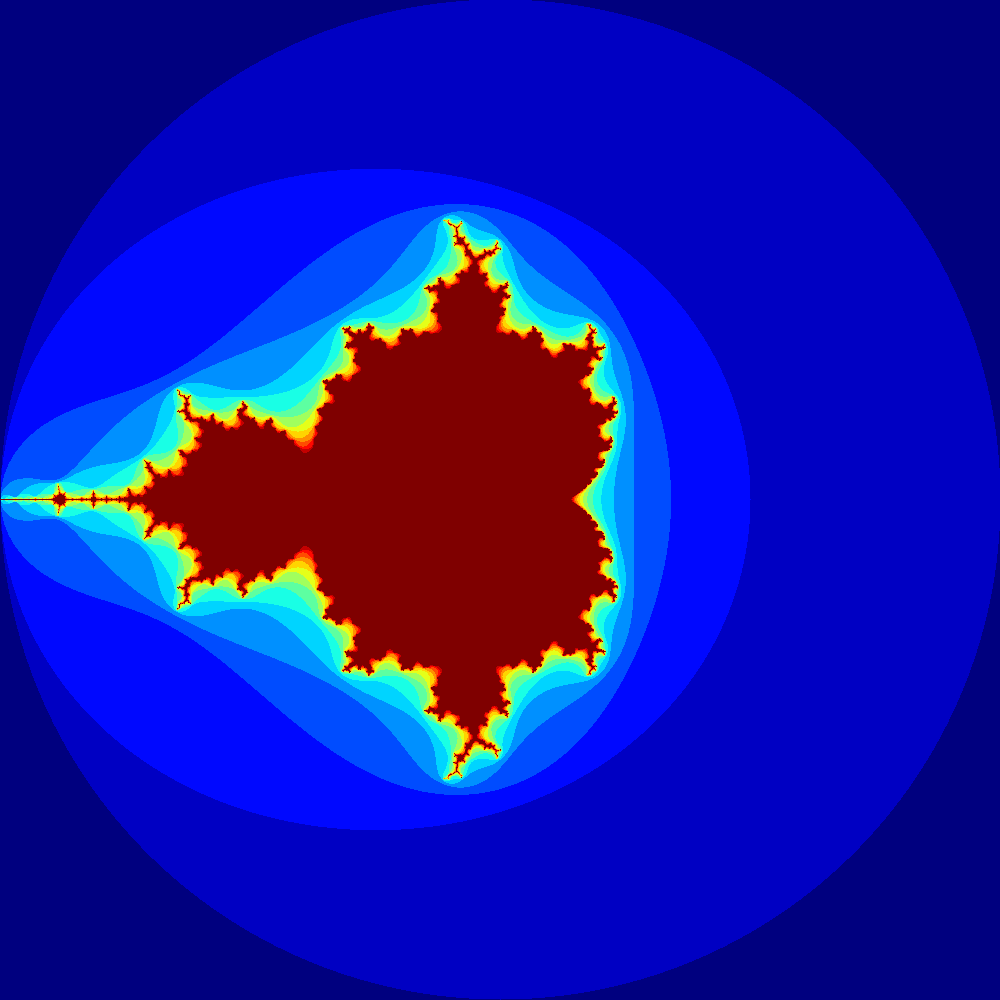
\includegraphics[width=0.2\textwidth]{img/F_0016.png}
        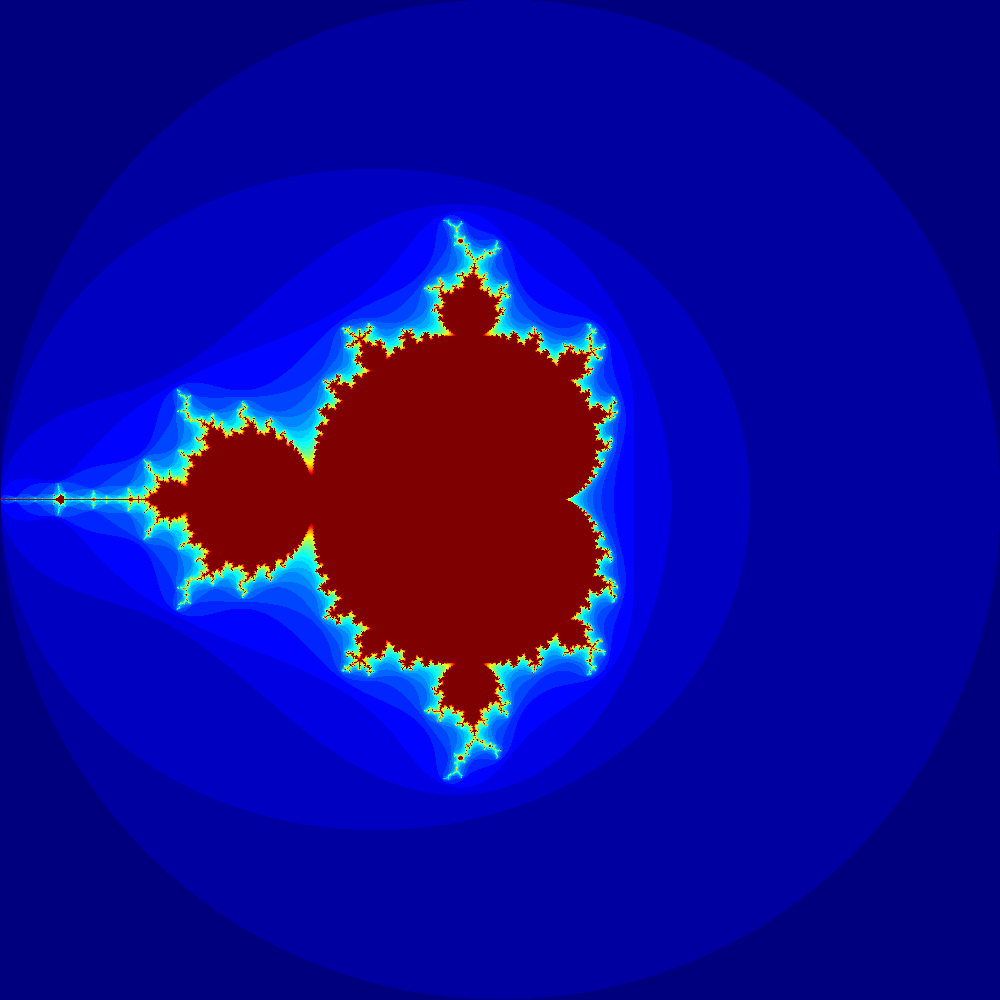
\includegraphics[width=0.2\textwidth]{img/F_0032.png}
        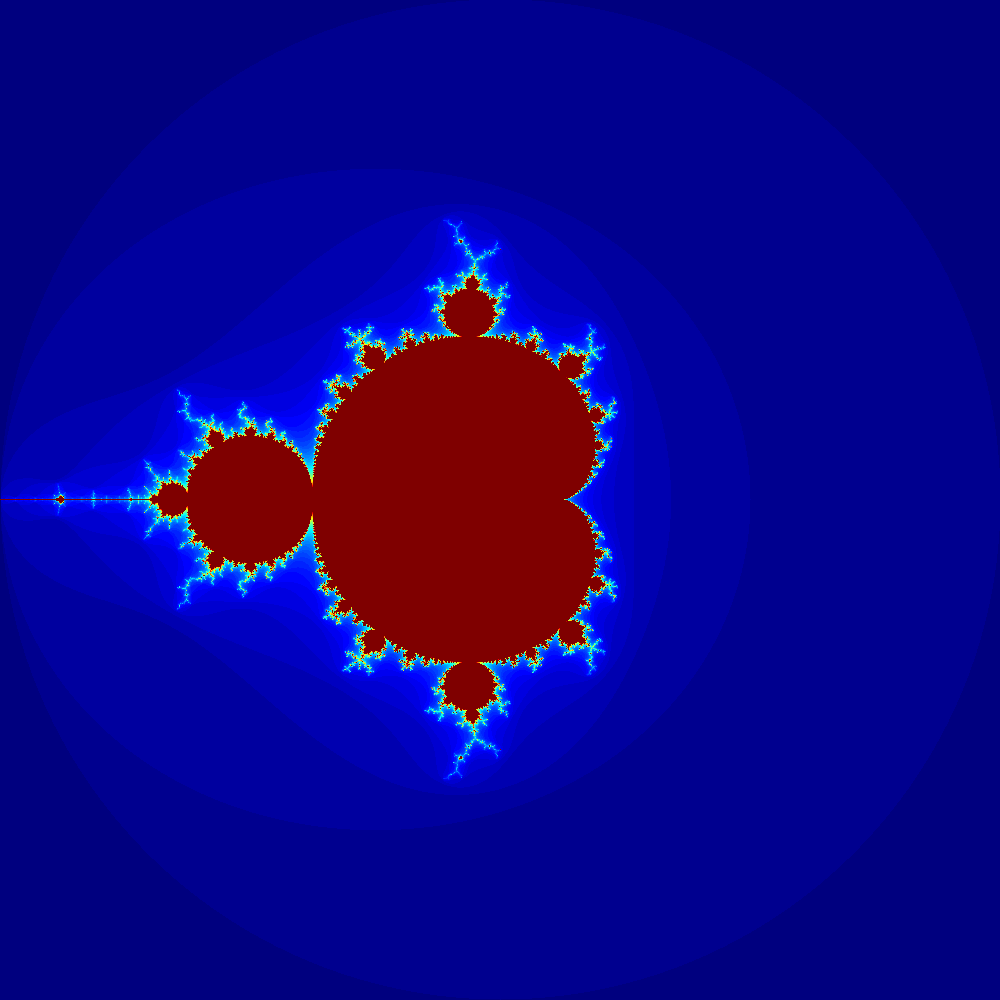
\includegraphics[width=0.2\textwidth]{img/F_0064.png}
        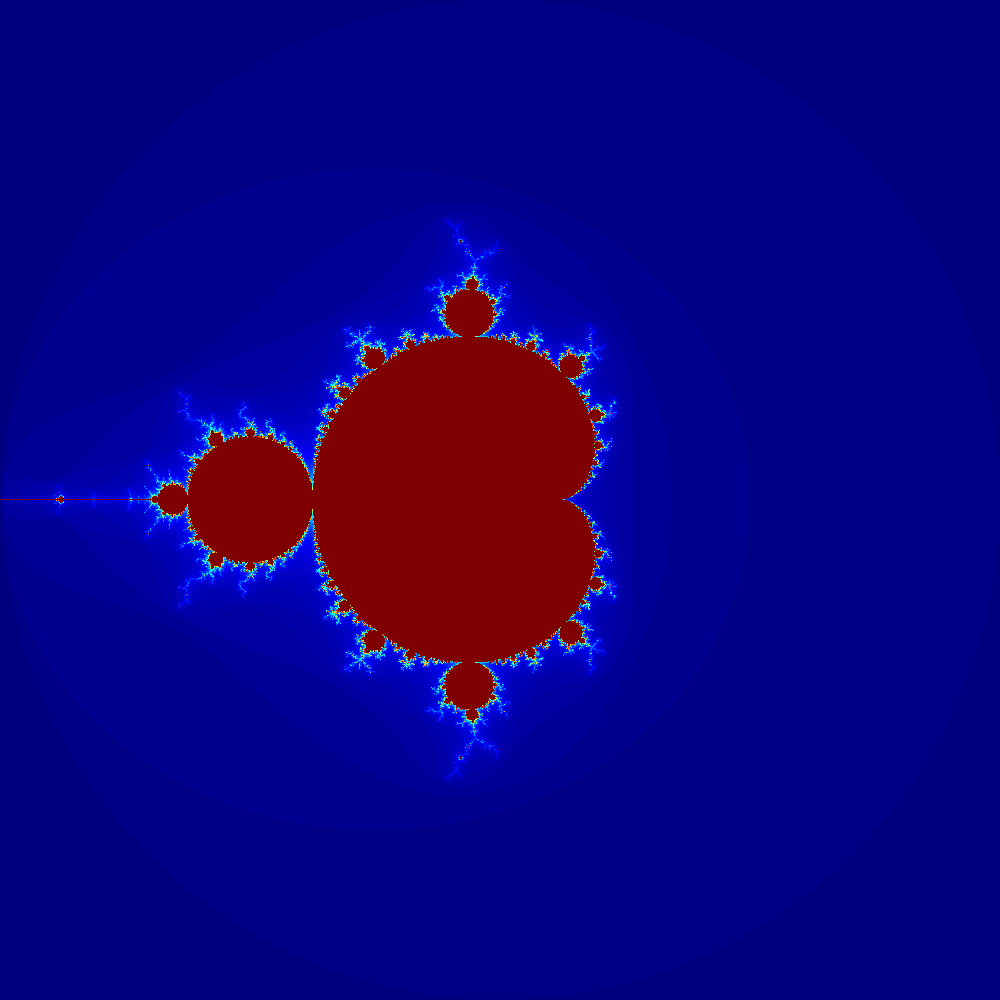
\includegraphics[width=0.2\textwidth]{img/F_0128.png}
        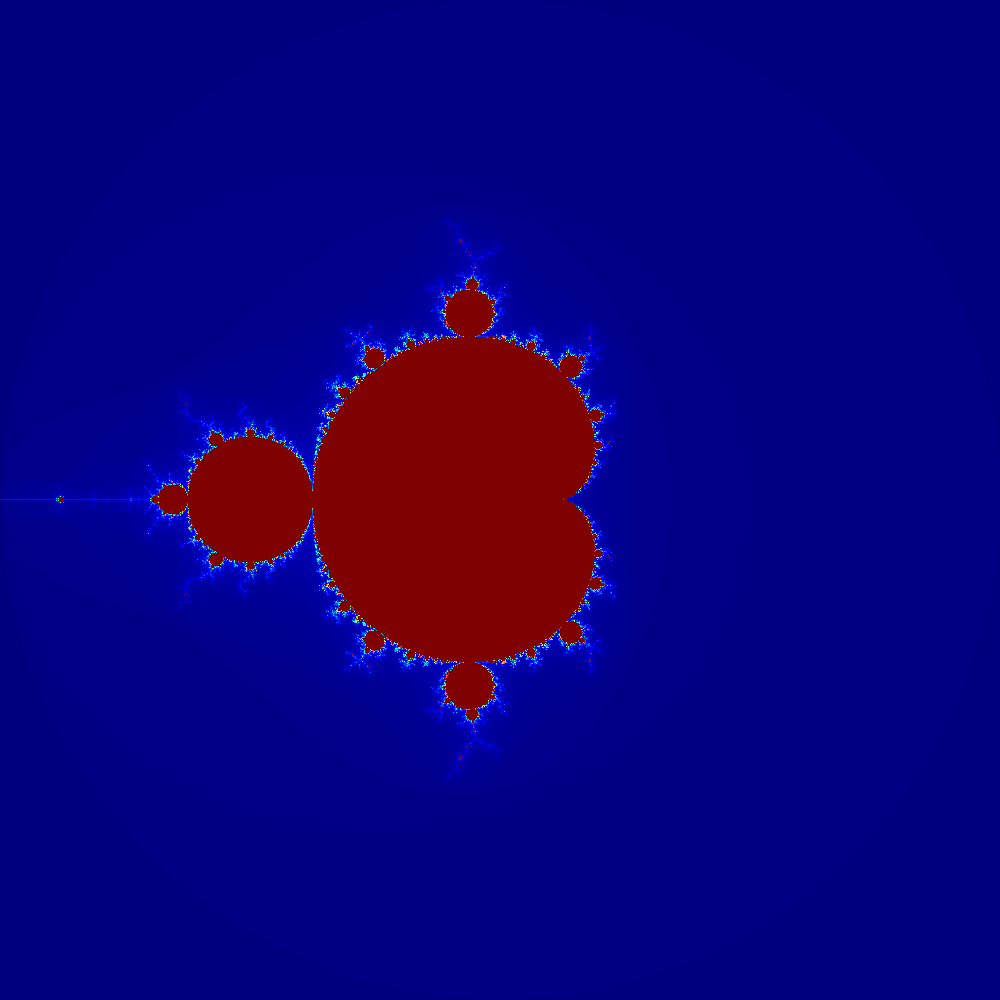
\includegraphics[width=0.2\textwidth]{img/F_0256.png}
        \caption{Evolution of Mandelbrot Set from 2 to 256 iterations}
        \label{fig:mandelbrot}
    \end{figure}

\subsection{Region Variation}
We also explored how varying the region of computation in the complex plane affects the execution time and the resulting fractal patterns. This section provides insights into the relationship between the complexity of the region and the computational effort required.

\subsubsection{Zone Visualization}

\begin{figure}[ht]
    \centering
    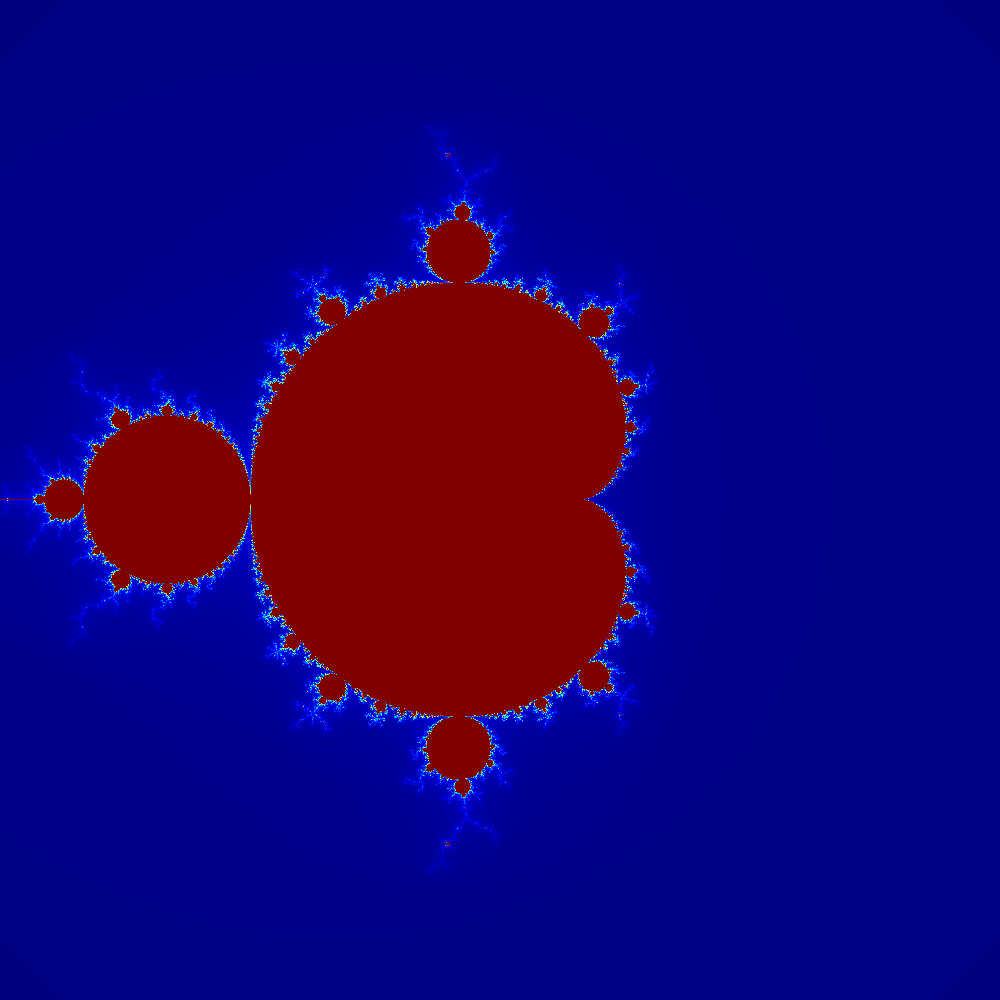
\includegraphics[width=0.2\textwidth]{img/F_ones.png}
    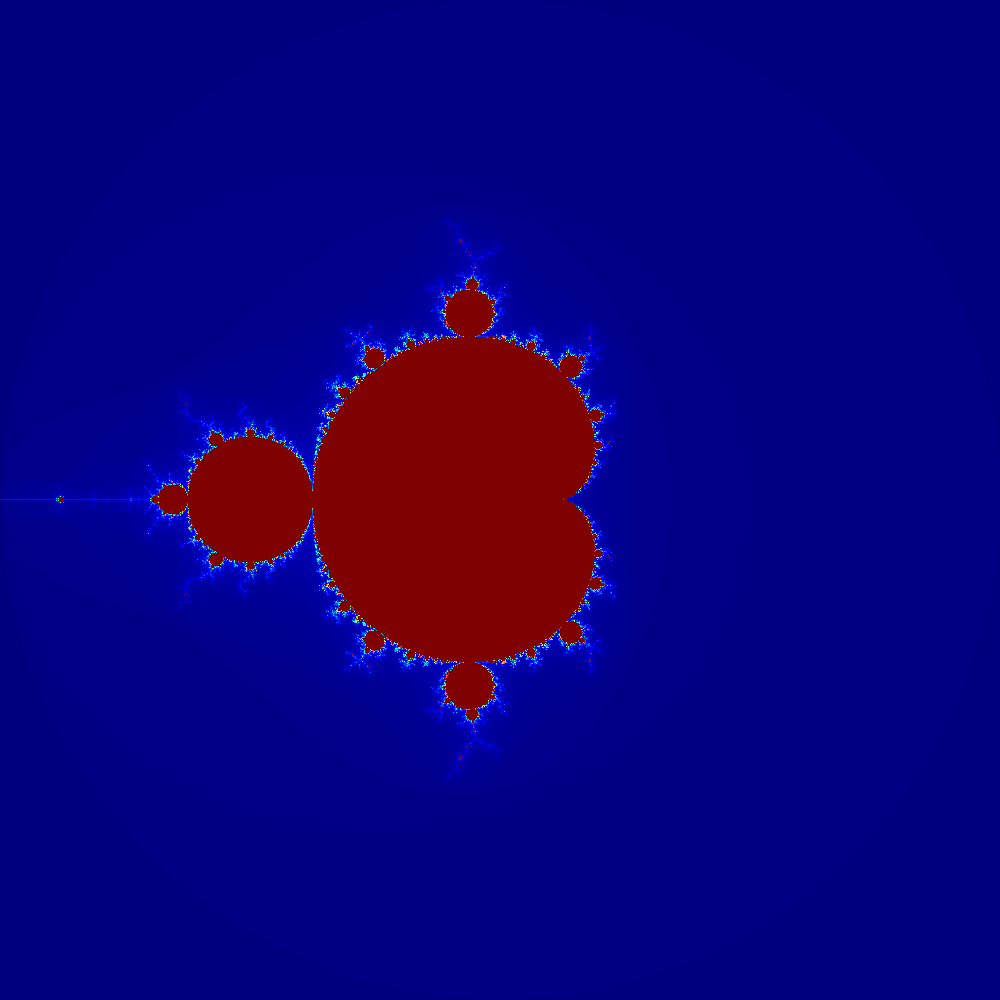
\includegraphics[width=0.2\textwidth]{img/F_twos.png}
    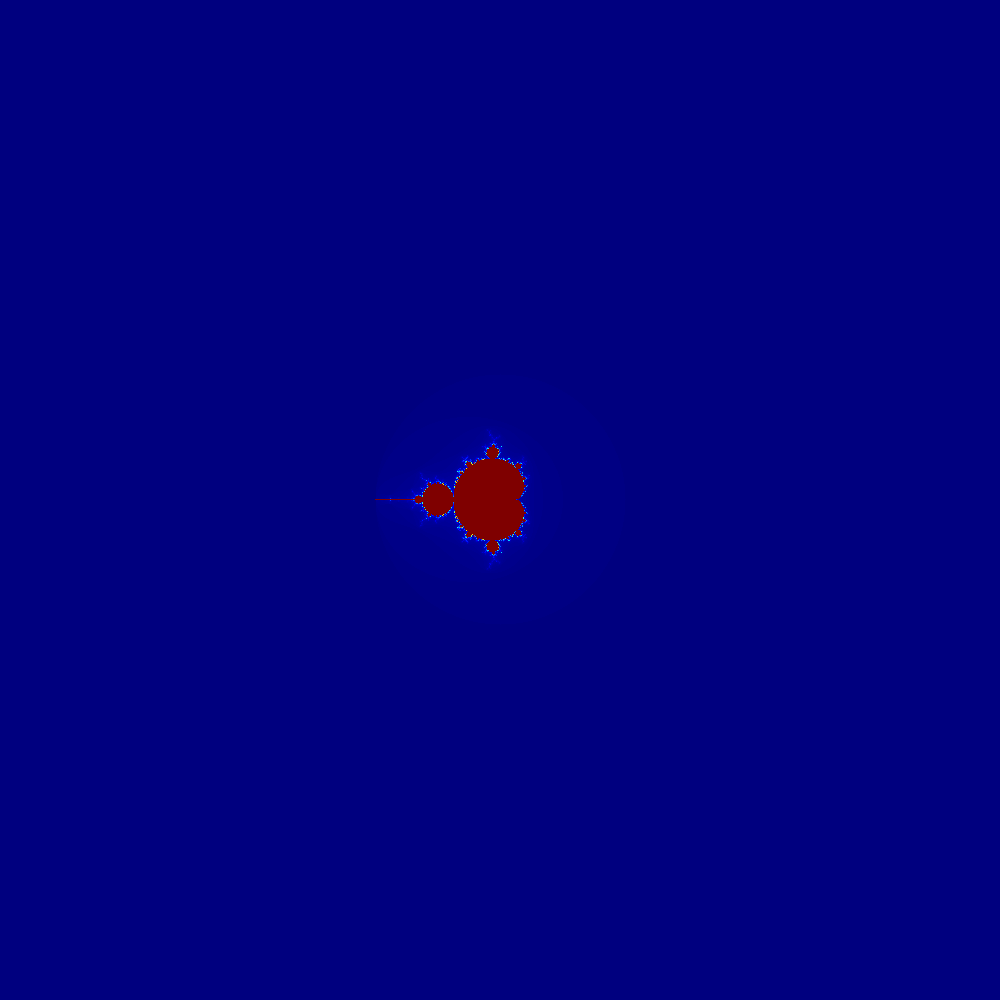
\includegraphics[width=0.2\textwidth]{img/F_eights.png}
    \caption{Different regions of computation}
    \label{fig:mandelbrot}
\end{figure}

\subsubsection{Time Variation}

\begin{itemize}
    \item Region: -1.5 -1.5 1.5 1.5, Time: 0.0705245 seconds
    \item Region: -2 -2 2 2, Time: 0.0479166 seconds
    \item Region: -8 -8 8 8, Time: 0.00753379 seconds
\end{itemize}

\section{Discussion}
The results indicate an initial trend of decreasing execution time with increased thread counts, demonstrating the efficiency of parallel computing. However, the slight increase in execution time beyond 64 threads can be attributed to several factors, including thread management overhead, memory bandwidth limitations, and the inherent complexity of the algorithm.

    The overhead of managing a large number of threads can outweigh the benefits of parallelization. As more threads are added, the cost of creating, scheduling, and synchronizing these threads becomes significant. This phenomenon is often observed in parallel computing and is a critical factor in determining the optimal number of threads for a specific computation.

    Memory bandwidth limitations also play a role. With more threads, the contention for memory access increases, potentially leading to bottlenecks that impede overall performance. This is particularly relevant for algorithms like the Mandelbrot set computation, where each thread requires access to memory for reading and writing data.

    Furthermore, the complexity of the Mandelbrot set itself influences execution time. Regions with more complex patterns require more iterations to resolve, leading to longer computation times. This aspect was evident in our experimentation with different computation regions, where more intricate areas of the set demanded more computational resources.

\section{Conclusion}
The exploration of the Mandelbrot set using OpenMP underscores the potential and challenges of parallel computing in handling complex mathematical computations. This report concludes with a reflection on our findings, emphasizing the balance between computational resources and efficiency, and suggesting avenues for future research in this domain.

\end{document}
